\chapter{Abwicklung von Sicherheitsrisiken}

%Systemplanung und Projekte Entwicklung von Felix Schwab, Ingridschwab-Matkovits
%https://searchcompliance.techtarget.com/definition/risk-management#:~:text=Risk%20management%20is%20the%20process,errors%2C%20accidents%20and%20natural%20disasters.
\section{Risikomanagement im Bereich Anmeldesysteme}
Das Risikomanagement sollte für jedes Unternehmen eine Top-Priorität sein. Durch dieses Verfahren kann man zukünftige Bedrohungen abschätzen und sich dazu Bewältigungsstrategien überlegen. Eine Firma muss im Vorhinein sich überlegen welche Risiken eintreten können. Diese Bedrohungen können durch viele verschiedene Ereignisse eintreten durch beispielsweise Naturkatastrophen, rechtliche Verpflichtungen, Managementfehler und sonstige Unfälle.
Mit der Planung einer neuen oder ausbaubaren IT-Infrastruktur sollte unbedingt das Risikomanagement in Betracht gezogen werden. Die Firma muss versuchen Risiken zu vermeiden oder diese bis zu einem gewissen Grad zu vermindern. 

\begin{center}
\begin{figure}[h]
    \centering
    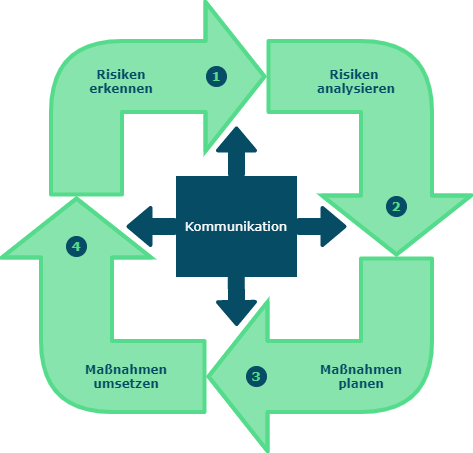
\includegraphics[width=10cm]{Risikomanagement_zyklus.png}
    \caption{Liefermodelle von Cloud Computing}
\end{figure}
\end{center}

\newpage

%BILD EINFUEGEN
\subsection{Ablauf Risikomanagement}
\begin{enumerate}
    \item Risiken identifizieren
    \item Risiken analysieren
    \item Maßnahmen planen
    \item Maßnahmen umsetzen
\end{enumerate}


\subsection{Grundbegriffe Risikomanagement}
%Systemplanung und Projekte Entwicklung von Felix Schwab, Ingridschwab-Matkovits
\subsubsection{Risiko}
Unter dem Begriff Risiko assoziiert man im Bereich IT-Sicherheit die Schadenshöhe, wenn ein bestimmtes Ereignis eintritt. Diese Ereignisse haben einen negativen Effekt auf das Unternehmen. Sie tragen dazu bei, dass materielle oder immaterielle Schäden auftreten können oder sogar Arbeitsprozesse abstoppen.
\\

%Systemplanung und Projekte Entwicklung von Felix Schwab, Ingridschwab-Matkovits
\subsubsection{Maßnahme}
Eine Maßnahme ist eine Handlung, die es ermöglicht ein Risiko zu umgehen oder es einzugrenzen, hier spricht man von der Schadensminimierung. 

%https://www.bva.bund.de/DE/Services/Behoerden/Beratung/Beratungszentrum/GrossPM/s-o-s_handbuch/stda_sos-kap8_risikomgmt.html
\subsection{Ziele des Risikomanagements}
Die Ziele die ein Unternehmen im Blick haben muss sind:
\begin{enumerate}
	\item \textbf{Risiken ausführlich identifizieren:} Die Firma darf keinesfalls essentielle Risiken nicht übersehen.
	\item \textbf{Risiken geeignet bewerten:} Bedrohungen / Risiken sollen in Hinsicht auf die Eintrittswahrscheinlichkeit, möglichen Auswirkungen und auf zeitliche Nähe eingeschätzt werden. Zusätzlich sollen diese darauffolgend mit dieser Betrachtungsweise bewertet werden.
	\item \textbf{Gleichgewicht zwischen Analyse und Umsetzung} Hier wird versucht eine Balance zu finden zwischen Risiken analysieren und dem Auftraggeber und der Projektleitung diese aufzuzeigen, zum anderen muss beachtet werden, das Gegenmaßnahmen getroffen werden.
	\item \textbf{Minimierung von Risiken} Ein Risiko an sich, kann nicht verändert werden. Das Unternehmen kann lediglich durch ein aktives entgegenwirken, die Wahrscheinlichkeit des Eintretens vermindern oder verhindern.
	\item \textbf{Kommunikation} Dieses Ziel gibt an das die Risiken dem Auftraggeber rechtzeitig übermittelt werden.
	\item \textbf{Überwachung} Alle diese Ziele müssen für neue oder schon bekannte Risiken immer wieder zyklisch durchgeführt werden. 
\end{enumerate}

\subsection{Umsetzungsprozesse}
Im Risikomanagement existieren unterscheidet man grundsätzlich zwischen zwei Arten von Umsetzungsprozessen, einmal initiale Prozesse und laufende Prozesse.
Diese beiden Prozesse werden auch als Aufbau Risikomanagement und als laufendes Risikomanagement bezeichnet.

\subsection{Aufbau Risikomanagement}
\subsubsection{Verantwortung und Budget}
Bei der Aufbereitung des Risikomanagements müssen vorher die Rollen jeder einzelnen Personen die Einfluss auf das Projekt besitzen festgelegt werden. Es wird eine Stakeholderanalyse durchgeführt.
Zusätzlich muss ein Budget festgelegt werden das für die Bewältigung eines Risikos eingesetzt wird. Hier muss gegenübergestellt werden wie viel Kosten entstehen falls das Risiko eintritt und wie viel die Bewältigung kostet.

\subsubsection{Kommunikation und Prozesse}
Es ist zu definieren, dokumentieren und kommunizieren wie oft und in welchen Abständen Mitarbeiter oder Stakeholder zu eine Einschätzung zu einem gewissen Risiko abgeben sollen. 
WIRD NOCH ERWEITERT

%https://www.business-wissen.de/hb/risiken-identifizieren/#:~:text=Insofern%20ist%20die%20Identifikation%20von,Sch%C3%A4den%20unvorhergesehen%20und%20%C3%BCberraschend%20eintreten.
\subsubsection{Risikoidentifikation}
Alle Risiken zu identifizieren die möglicherweise auftreten können, kann sich als sehr schwer erweisen. Es können etwaige Risiken auftreten, von denen noch nichts bekannt war oder die man nicht in Betracht gezogen hat. Aus diesen Gründen ist die Identifikationsphase eine sehr wichtige. Sie muss sorgfältig durchgeführt werden und mit verschiedenen Ansätzen abgewickelt werden. Fortlaufend sollte deswegen regelmäßig überprüft werden ob sich Risiken verändern oder möglicherweise hinzukommen.
\\

%Methoden gefunden: Im Syp Buch
%https://de.wikipedia.org/wiki/Risikoidentifikation#:~:text=Als%20Methoden%20kommen%20f%C3%BCr%20bestehende,oder%20die%20Delphi%2DMethode%20ermitteln.
\subsubsection{Risiken und Potenzielle Risiken}
Die Risikoidentifikation beschäftigt sich mit zwei Arten von Risiken einmal die bekannten Risiken und die potenziellen Risiken. Folgende Methoden können zur Bewältigung angewandt werden:
\begin{enumerate}
    \item \textbf{Methoden um bestehenden/bekannte Risiken zu identifizieren}
    \begin{itemize}
        \item Einsatz von Checklisten
        \item SWOT-Analyse
        \item Befragungen von erfahrenen Mitarbeitern
        \item Befragungen von Experten mit spezifischen Fachwissen
    \end{itemize}
    \item \textbf{Methoden um Potenzielle Risiken zu identifizieren}
    \begin{itemize}
    	\item Brainstorming
    	\item Delphi-Methode
    	\item Mindmapping
    	\item Morphologischer Kasten
    	\item Brainwriting (bzw. 6-3-5 Methode)
    \end{itemize}
\end{enumerate}

%https://de.wikipedia.org/wiki/Risikoidentifikation#Checklisten_und_Mitarbeiterbefragungen
\paragraph{Einsatz von Checklisten}
Bei dieser Methode werden standardisierte Checklisten verwendet. Diese sollen einem Unternehmen aufzeigen welche Risiken zu beachten sind, wenn es um die Informationssicherheit geht. Es besteht nur ein Nachteil, es werden nicht alle für das eigene Unternehmen relevanten Risiken genannt.

%https://smallbusiness.chron.com/security-swot-analysis-40526.html
\paragraph{SWOT-Analyse}
SWOT(Strengths, Weaknesses, Opportunities, Threats) ist eine Methode verschiedene Faktoren zu analysieren. 
Durch infrage stellen der Stärken (Strengths) und Schwächen (Weaknesses) einer Firma kann man unternehmensinterne Faktoren identifizieren.
\subparagraph{Stärken}
Eine Stärke von einem Betrieb kann beispielsweise, die Verwendung von Firewalls und Anti-Virus Programmen sein. Regelmäßiges Ändern von Passwörtern der Mitarbeiter eines Betriebs kann verhindern, dass eine unternehmens-fremde Person oder Unternehmen keinen Zugriff auf die von der Firma genutzten Systeme haben kann.

\subparagraph{Schwächen}
Schwächen müssen erkannt werden und mit Gegenmaßnahmen behoben werden.
Wenn beispielsweise das Unternehmen nicht viel in die Sicherheit eines Systems investiert hat, kann es passieren das möglicherweise eine Data Breach(Datenabfluss) auftreten kann. Die Behebung des Problems wäre das alle Firmengeräte einen Virenschutz und einen VPN-Dienst nutzen.

Durch hinterfragen von Möglichkeiten (Opportunities) und Bedrohungen (Threats) werden externe Faktoren gefunden, die mit einfließen.

\subparagraph{Möglichkeiten}
In der heutigen Zeit gibt es im Bereich der IT sehr viele verschiedene Anbieter für die unterschiedlichsten Services, wie z.B. Cloud-Services.
Diese Services nehmen dem Unternehmen die Arbeit ab ein eigenes Serversystem aufzubauen und zu verwalten. Dementsprechend wird der Firma geholfen ein Risiko zu vermindern und nimmt dem Betrieb einen sehr großen Aufwand ab. 

\subparagraph{Bedrohungen}
In diesem Bereich muss überlegt werden was gemacht werden soll wenn ein Ausnahmefall, beispielsweise eine Naturkatastrophe oder ein Hacking-Angriff, eintritt. Somit muss überlegt werden, wie im Vorhinein gehandelt werden soll. Es muss überlegt werden, wie man die Daten von dem Unternehmen sichert, dass kann durch verschiedene Backup-Strategien sichergestellt werden.


%https://de.wikipedia.org/wiki/Risikoidentifikation#Checklisten_und_Mitarbeiterbefragungen
\paragraph{Befragungen}
Bei diesen Umfragen werden entweder erfahrene Mitarbeiter oder Experten mit gewissen Fachwissen befragt. Der Vorteil bei der Befragung von Mitarbeitern ist, dass sie eher interne Unternehmensrisiken identifizieren. Bei dem Einstz von Experten werden eher externe unternehmens bedrohliche Risiken erkannt. Befragungen können in einer digitalen, schriftlichen oder mündlichen Arten statt finden.
Wichtig ist es bei diesen Befragungen die Fragen genau beschrieben, sinnvoll und auf das Unternehmen angepasst sind.

%Buch S. 38
\paragraph{Brainstorming}
Hier versammeln sich eine Gruppe von unternehmensinternen Personen bestehend aus bevorzugter Weise aus fünf bis sieben Personen. 
Beim Brainstorming Prozess werden Vorschläge und Ideen nur verbal geäußert und danach dokumentiert. Eine Person der sogenannte Moderator leitet diesen Kommunikationsprozess. Vorzugsweise sollte dieser Vorgang nur zehn bis maximal zwanzig Minuten andauern.
Die Bewertung der erhobenen Ideen / Vorschlägen darf nicht gleichzeitig mit der Erhebung ablaufen und dürfen deswegen nur in einer zweiten Phase abgehalten werden.

Es gibt gewisse Regeln die zu beachten sind:
\begin{itemize}
	\item Keine Barrieren, d.h. man kann alles Vorschlagen, auch nicht umsetzbare oder absurde Ideen. Keine Idee ist zu extrem.
	\item Keine Diskriminierung, damit ist gemeint, dass kein Teilnehmer für eine geäußerte Idee kritisiert werden soll. Diese Regel ist sehr wichtig, da es sonst den kreativen Prozess stört oder sogar verhindert.
\end{itemize}

%Buch S. 38
\paragraph{Brainwriting (6-3-5 Methode)}
Bei dieser Methode gibt es sechs Personen die sich zusammensetzen, jeder Teilnehmer soll dann jeweils 3 Ideen schriftlich festhalten, in einer Zeit von ungefähr 5 Minuten.
Als nächster Schritt wird dann das Schriftstück in der Runde verteilt, dass kann entweder in eine Richtung weiter gegeben werden oder sie werden durchgemischt und dann verteilt. 
Als Ergebnis dieser Methode sollten nach 30 Minuten 108 Ideen aufgeschrieben worden sein.
Der Vorteil dieser Methode ist, dass alle Ideen dokumentiert worden sind und die Ergebnisse deshalb in einer schriftlichen Form vorhanden sind.

%Buch S. 41
\paragraph{Delphi-Methode}
Bei der Delphi-Methode wird eine Problemstellung oder ein Risiko von einer Gruppe aus verschiedenen und nicht voneinander abhängigen Experten bzw. Fachleuten bearbeitet. 
Jeder Teilnehmer erarbeitet einen Lösungsansatz zu dem gestellten Risiko auf einem Schriftstück.
Die Ausarbeitungen werden eingesammelt und anonymisiert weitergegeben.
Der erhaltene Lösungsansatz soll jetzt kritisiert werden, d.h. falls die Person Denkfehler oder falsche Ansätze verwendet. Aus dieser Bearbeitung, soll man für das eigene Konzept Ideen oder Änderungen finden und integrieren.
Dieser Prozess soll mehrere male wiederholt werden, so dass die Gruppe eine gemeinsame Lösung beschließt.
Die Anonymität spielt bei der Methode eine große Rolle und trägt dazu bei, dass jeder Teilnehmer kreative und alternative Standpunkte einnimmt.
Der Vorteil diese Methode anzuwenden ist, dass unabhängige Fachleute eingesetzt werden und diese über einen größeren Zeitraum an dieser Problematik arbeiten.
Ein daraus folgender Nachteil ist ein hoher Zeit- und Organisationsaufwand.


\paragraph{Mindmapping}
Das Mindmapping ist eine Methode die angewandt wird um Assoziationen zu einem Thema grafisch darstellen.
WIRD NOCH ERWEITERT

\paragraph{Morphologischer Kasten}
Beim morphologischen Kasten werden viele verschiedene Aspekte oder gewisse Merkmale von einer Lösung in eine systematische Reihenfolge angeordnet. Diese Technik soll dazu führen zu erkennen welche ideale Kombination für die Risikobewältigung, verwendet werden kann.
WIRD NOCH ERWEITERT

\subsection{Laufendes Risikomanagement}
IN PROGRESS

FAZIT ZU MEINEM PART